\chapter{Хаос в открытых квантовых системах}\label{ch:ch3}

Взаимосвязь между квантовыми системами и их классическими аналогами (в частности, среднеполевые приближения) являются ключевой проблемой теории квантового хаоса \cite{Stockmann2006}. 
До настоящего времени данная связь анализировалась в основном с точки зрения спектральных характеристик квантовых гамильтонианов. 
В данном контексте одной из самых важных вех в развитии квантового хаоса являлось установление связи между спектральной статистикой и переходами от регулярной динамики к хаотической (и наоборот) в фазовом пространстве соответствующих классических систем \cite{Stockmann2006}.

Бифуркационный анализ \cite{Poincare1885} является одним из основных подходов изучения нелинейной динамики и ее приложений \cite{Kuznetsov2004}.
Применение бифуркационного анализа в сфере квантовой физики долгое время рассматривалось только в контексте изолированных систем  "---  гамильтонов хаос, спектральные характеристики которого в квантовых системах к настоящему времени являются очень хорошо изученными \cite{Casati1979, Gutzwiller1990}.
Квантовые следы бифуркаций, то есть существенных изменений в структуре фазового пространства классических гамильтоновых систем при небольшом изменении параметра(ов), также исследовались в работах \cite{Hines2005, Santos2006, Nemes2006}. Здесь было обнаружено, что классические бифуркации типа «вилка» и Андронова"--~Хопфа \cite{Wiggins2013} в среднеполевых моделях связаны с резкими изменениями запутанности основного состояния в соответствующих квантовых моделях.
Кроме этого, в работе \cite{Zibold2010} было обнаружено, что бифуркация типа «вилка» соответствует переходу от динамики Раби к динамике Джозефсона в экспериментах с рубидиевым конденсатом Бозе"--~Эйнштейна.

Дальнейшее применение бифуркационного анализа к открытым квантовым системам в связке с соответствующими среднеполевыми моделями будет способствовать развитию теории диссипативного квантового хаоса. 
В случае открытых систем бифуркации могут иметь более серьёзные последствия, чем в гамильтоновом случае, потому что они будут влиять на стационарное состояние системы, а не только на конкретное собственное состояние изолированной системы.
Однако, существуют значительные трудности в построении среднеполевых приближений для открытых квантовых систем.

В недавней работе \cite{Ivanchenko2017} было обобщено понятие бифуркации для случая квантовых диссипативных систем.
Обычно квантовые бифуркации визуализируются путём вычисления квазиклассических распределений фазового пространства, типа Хусими или Вигнера \cite{Stockmann2006}, структурные изменения которых с изменением параметра воспроизводят бифуркации в классическом фазовом пространстве. 
Например, квантовая бифуркация удвоения периода рассматривается как переход от унимодального к бимодальному распределению Хусими \cite{Hartmann2017, Wang2018}.
В работе \cite{Ivanchenko2017}, используя многочастичную модель квантового димера было показано, что асимптотическая матрица плотности открытой системы может быть использована для построения бифуркационной диаграммы классического типа, которая может быть связана с классической динамикой в среднеполевом приближении рассматриваемой квантовой модели.
Такой подход позволил преодолеть технические ограничения при вычислении распределения Хусими для систем с большим числом состояний.
В итоге были обнаружены квантовые аналоги некоторых классических типов бифуркаций "--- седлоузловая, типа «вилки», а также сценарий перехода к квантовому хаосу через каскад бифуркаций удвоения периода.

Другим важным направлением развития теории диссипативного квантового хаоса является создание инструментов для его количественной оценки.
Одна из основополагающих концепций теории динамического хаоса заключается в том, что сложная хаотическая динамика возникает из-за локальной нестабильности, которая заставляет две изначально близкие траектории расходиться. 
Это расхождение обычно количественно оценивается с помощью показателей Ляпунова "--- мощного инструмента для количественной оценки динамического хаоса.
Попытки обобщения показателя Ляпунова на квантовую динамику предпринимаются давно. 
В большинстве исследований рассматриваются случаи гамильтоновых систем, где впервые была создана спектральная теория квантового хаоса \cite{Haake2018}.
Соответствующие обобщения варьируются от ранних идей использования функций квазивероятности и определения квантовых показателей Ляпунова в терминах «расстояния» между ними \cite{Toda1987, Haake1992, Manko2000} до самых недавних достижений, основанных на вневременных корреляционных функциях \cite{Rozenbaum2017, Liao2018, ChavezCarlos2019}.

Подходы, пытающиеся согласовать свойства спектров генераторов диссипативной квантовой эволюции (линдбладианов) \cite{book2007} или спектров асимптотической матрицы плотности \cite{Hartmann2017, Ivanchenko2017, Prosen2013} с переходами между регулярным и хаотическим режимами в соответствующих среднеполевых моделях, дали некоторые интересные результаты. Однако, область количественной оценки диссипативного квантового хаоса все ещё остаётся малоизученной.

Также отдельный интерес вызывают не только теоретические характеристики квантового диссипативного хаоса, но и квантификаторы динамики системы, которые можно получить из реального физического эксперимента. 
В качестве модели в данном контексте можно рассматривать  квантовый электродинамические (КЭД) резонатор, в экспериментальной реализации которого можно наблюдать за эмиссией фотонов \cite{Walther2006, Arakawa2015}.
Последние достижения в данной области позволяют, например, изготовить полупроводниковую квантовую точку и встроить ее в микрополость \cite{Arakawa2015}. 
Квантовая точка может иметь от двух до четырёх уровней энергии, a взаимодействие между модами резонатора и точечными экситонами также может быть настроено \cite{Reithmaier2004, Hennessy2007}. 
Небольшое количество энергетических уровней делает квантовые точки хорошими кандидатами для реализации кубитов, в то время как взаимодействие между ними может регулироваться при помощи резонатора.

В разделе \cref{sec:ch3/dimer} описывается модель взаимодействующих бозонов в открытом квантовом димере с периодической модуляцией. Для данной системы существует среднеполевое приближение, что позволяет провести сравнение квантовой и классической (в пределе бесконечного числа частиц) динамики. В контексте квантового димера будет обнаружен квантовый аналог бифуркации Неймарка"--~Сакера и введено новое квантовое обобщение показателя Ляпунова на основе метода квантовых траекторий.

В разделе \cref{sec:ch3/neimark}, используя модель периодически модулированного открытого квантового димера, исследуется квантовая бифуркация Неймарка"--~Сакера. 
Её классический аналог "--- рождение тора (инвариантной кривой в сечении Пуанкаре) из-за неустойчивости предельного цикла (неподвижной точки отображения Пуанкаре).
Квантовая система демонстрирует переход от унимодального к стробоскопическому распределению в форме бублика, как для распределений Хусими \cite{Stockmann2006}, так и для наблюдаемых величин, вычисленных для отдельных квантовых траекторий. 
При этом спектральные свойства отображения Флоке для квантового димера изменяются аналогично классическому случаю "---  пара комплексно-сопряженных собственных значений приближается к единичной окружности. 
Динамика отдельных квантовых траекторий на «квантовом торе» позволяет количественно определить число вращения.
Также будет показано, что бифуркация чувствительна к количеству квантовых частиц, которое также можно рассматривать как управляющий параметр.

В разделе \cref{sec:ch3/le} вводится обобщение квантового показателя Ляпунова для диссипативных систем на основе количественного определения расходимости изначально близких квантовых траекторий.
Введенный квантовый показатель Ляпунова будет использован для выявления сложной структуры регулярных и хаотических областей, а также различных бифуркаций в модели квантового димера.

В разделе \cref{sec:ch3/pwtd} будет предложен экспериментально релевантный подход определения типа динамики открытого квантового резонатора с периодической модуляцией. Будет продемонстрировано, что хаотические режимы проявляют промежуточную степенную асимптотику в распределении времён ожидания фотона. Это распределение можно получить, отслеживая испускание фотонов с помощью однофотонного детектора без нарушения динамики внутри резонатора.

В разделе \cref{sec:ch3/csp} численно исследуется модель открытого квантового резонатора внутрь которого помещён одним спин, что позволяет регулировать степень хаотизации динамики системы в терминах квантовых показателей Ляпунова и статистики времён между последовательными излучениями фотонов.

В разделе \cref{sec:ch3/results} представлены основные выводы по данной главе.

\section{Открытый квантовый димер}\label{sec:ch3/dimer}
Модель состоит из \(N\) неразличимых взаимодействующих бозонов, которые перемещаются между двумя узлами периодически модулируемого димера. 
Данная модель является популярной в теоретических исследованиях \cite{Vardi2001, Trimborn2008, Poletti2012} и имеет экспериментальную реализацию \cite{Gross2010, Tomkovic2017}. Кроме этого, в данной модели были обнаружены различные хаотические и регулярные режимы \cite{Hartmann2017, Ivanchenko2017, Carlo2017, Wang2018}. 

\subsection{Квантовая модель}\label{subsec:ch3/dimer/quantum}

Унитарная часть уравнения Линдблада \labelcref{eq:GKSL_base, eq:GKSL_lindbladian} задается следующим гамильтонианом:
\begin{equation}
	\label{eq:dimer_H}
	\begin{gathered}
		H(t) = -\mathcal{J} \left(b^\dagger_1 b_2 + b^\dagger_2 b_1\right) + \frac{2 U}{N} \sum_{g=1,2} n_g \left(n_g - 1\right) + \varepsilon(t) \left(n_2 - n_1\right),
	\end{gathered}
\end{equation}
где первое слагаемое отвечает за перемещение бозонов между двумя узлами димера с коэффициентом \(\mathcal{J}\), второе слагаемое "--- за взаимодействие бозонов с силой \(U\), находящихся в  одном и том же узле и третье слагаемое "--- периодическая модуляция с функцией \(\varepsilon(t)\). 
Операторы \(b_j\) и \(b^\dagger_j\) соответствуют рождению и уничтожению бозона на сайте \(j\), \(n_j = b^\dagger_j b_j\) "--- оператор числа частиц на сайте \(j\).

В дальнейшем будут рассмотрены два типа периодической модуляции димера.
Непрерывная (C - Continuous) функция модуляции:
\begin{equation}
	\label{eq:dimer_mod_c}
	\begin{gathered}
		\varepsilon_{C}(t) = \varepsilon_{C}(t + T) = A \sin(\Omega t),
	\end{gathered}
\end{equation}
где \(T\) "--- период модуляции, \(A\) "--- амплитуда модуляции (разность энергий между сайтами димера), \(\Omega = 2 \pi / T\).
Второй тип модуляции "--- кусочно-постоянная (P - Piecewise):
\begin{equation}
	\label{eq:dimer_mod_p}
	\begin{gathered}
		\varepsilon_{P}(t) = \varepsilon_{P}(t + T) = \mu_0 + \mu_1 Q(t), \\
		Q(\tau) = 1, \quad 0 < \tau \le T/2, \\
		Q(\tau) = 0, \quad T/2 < \tau \le T,
	\end{gathered}
\end{equation}
где \(T\) "--- период модуляции, \(\mu_0\) и \(\mu_1\) "--- постоянная и переменная разница в уровне энергий между сайтами димера, \(Q(\tau)\) "--- периодическая функция, принимающая два значения.

Гильбертово пространство системы имеет размерность \(S = N + 1\) и каждое базисное состояние системы можно обозначить как число бозонов в первом сайте димера \( \lbrace \left|n\right>\rbrace\), где \(n = 0,\ldots,N\). Таким образом, размер системы задаётся количеством бозонов в димере.

Во второй части уравнения Линдбдлада \labelcref{eq:GKSL_base, eq:GKSL_lindbladian}, отвечающей за взаимодействие с окружающей средой, участвует только один эксперементально-релевантный \cite{Diehl2008, Kraus2008} диссипативный оператор (\(K=1\)), который действует между двумя сайтами димера. Данный диссипатор имеет вид:
\begin{equation}
	\label{eq:dimer_diss}
	\begin{gathered}
		V = ( b^\dagger_1 + b^\dagger_2) \left( b_1 - b_2 \right),
	\end{gathered}
\end{equation}
и синхронизирует динамику на сайтах димера за счёт рециркуляции антисимметричных противофазных состояний в симметричные и синфазные. Скорость диссипации \(\gamma\) является независимой от времени величиной.

При использовании метода квантовых траекторий (раздел \cref{sec:ch1/qj}) для каждой траектории \(\left| \psi_j(t) \right\rangle\) ( \(j\) - индекс) в момент времени \(t\) будут вычисляться следующие значения наблюдаемых "--- нормированного числа частиц в первом сайте димера:
\begin{equation}
	\label{eq:dimer_num_bosons}
	\begin{gathered}
		n_j(t) =  \frac{1}{N}\langle \psi_j(t)| b^\dagger_1 b_1 | \psi_j(t) \rangle,
	\end{gathered}
\end{equation}
и нормированной энергии:
\begin{equation}
	\label{eq:dimer_energy}
	\begin{gathered}
		e_j(t) = \frac{1}{N} \langle \psi_j(t)| H(t) | \psi_j(t) \rangle.
	\end{gathered}
\end{equation}

\subsection{Среднеполевое приближение}\label{subsec:ch3/dimer/meanfield}
В пределе бесконечного числа частиц \(N \to \infty\) в среднеполевом приближении модели квантового димера используются следующие спиновые операторы:
\begin{equation}
	\label{eq:dimer_meanfield_spin}
	\begin{gathered}
		\mathcal{S}_x = \frac{1}{2 N} \left(b^\dagger_1 b_2 + b^\dagger_2 b_1\right), \\
		\mathcal{S}_y = - \frac{i}{2 N} \left(b^\dagger_1 b_2 - b^\dagger_2 b_1\right), \\
		\mathcal{S}_z = \frac{1}{2 N} \left(b^\dagger_1 b_1 - b^\dagger_2 b_2\right), \\
	\end{gathered}
\end{equation}
чья эволюция рассматривается в представлении Гейзенберга \cite{Breuer2007}. 
В пределе бесконечного числа частиц коммутатором первых двух спиновых операторов можно пренебречь: \(\left[\mathcal{S}_x, \mathcal{S}_y\right] = i \mathcal{S}_z \stackrel{N\to\infty}{=} 0\) (так как является бесконечно малой порядка $\mathcal{O}(N^{-1})$). 
Это же свойство справедливо для всех остальных коммутаторов, полученных из разных перестановок спиновых операторов.
Заменяя спиновые операторы их математическим ожиданием \(\mathscr{S}_k = tr\left[\rho\mathcal{S}_k\right]\), можно получить следующую систему дифференциальных уравнений \cite{Hartmann2017}:
\begin{equation}
	\label{eq:dimer_meanfield_ode_spin}
		\left\{
		  \begin{array}{rl}
		    \frac{d \mathscr{S}_x}{dt} = & 2\varepsilon (t) \mathscr{S}_y - 8 U \mathscr{S}_z \mathscr{S}_y + 8 \gamma \left(\mathscr{S}_y^2+\mathscr{S}_z^2\right) \\
		    \frac{d \mathscr{S}_y}{dt} = & -2\varepsilon \left(t\right) \mathscr{S}_x + 8 U \mathscr{S}_x \mathscr{S}_z - 2 \mathcal{J} \mathscr{S}_z + 8\gamma \mathscr{S}_x \mathscr{S}_y \\
		    \frac{d \mathscr{S}_z}{dt} = & -2 \mathcal{J} \mathscr{S}_y - 8 \gamma \mathscr{S}_x \mathscr{S}_z
		  \end{array}
		\right.
\end{equation}	
В данной системе есть интеграл движения: \(\mathscr{S}^2 = \mathscr{S}_x^2 + \mathscr{S}_y^2 + \mathscr{S}_z^2\) и эволюция среднеполевой модели ограничена поверхностью сферы Блоха \cite{Nielsen2010}:
\begin{equation}
	\label{eq:dimer_meanfield_sphere}
	\left\{
	\begin{array}{rl}
		\mathscr{S}_x = & \frac{1}{2} \cos{\left(\varphi\right)}\sin{\left(\vartheta\right)}\\
		\mathscr{S}_y = & \frac{1}{2} \sin{\left(\varphi\right)}\sin{\left(\vartheta\right)}\\
		\mathscr{S}_z = & \frac{1}{2} \cos{\left(\vartheta\right)}
	\end{array}
	\right.
\end{equation}
Система дифференциальных, описывающих движение на данной сфере выглядит следующим образом:
\begin{equation}
	\label{eq:dimer_meanfield_ode_sphere}
	\left\{
	\begin{array}{rl}
		\dot{\vartheta} = & -2\mathcal{J}\sin{\left(\varphi\right)} + 4\gamma \cos{\left(\varphi\right)}\cos{\left(\vartheta\right)} \\
		\dot{\varphi} = & -2 \mathcal{J} \frac{\cos{\left(\vartheta\right)}}{\sin{\left(\vartheta\right)}} - 2\varepsilon\left(t\right) + 4U \cos{\left(\vartheta\right)} - 4\gamma\frac{\sin{\left(\varphi\right)}}{\sin{\left(\vartheta\right)}}
	\end{array}
	\right.
\end{equation}
Число бозонов в первом сайте димера вычисляется по формуле:
\begin{equation}
	\label{eq:dimer_meanfield_num_bosons}
	\begin{gathered}
		n=\frac{N}{2}(1+\cos{\left(\vartheta\right)}).
	\end{gathered}
\end{equation}
Данная классическая нелинейная система \cref{eq:dimer_meanfield_ode_sphere} будет играть опорную роль и результаты полученные для неё будут сравниваться с результатами квантовой системы, описанной в разделе \cref{subsec:ch3/dimer/quantum}.

\section{Квантовая бифуркация Неймарка"--~Сакера}\label{sec:ch3/neimark}

В данном разделе изучается квантовая бифуркация Неймарка"--~Сакера, классическим аналогом которой является рождение тора (инвариантной кривой в стробоскопическом отображении Пуанкаре) из-за неустойчивости предельного цикла (неподвижная точка отображения Пуанкаре) \cite{Kuznetsov2004}.
На примере экспериментально релевантной модели открытого квантового периодически модулированного димера (раздел \cref{subsec:ch3/dimer/quantum}), будет показано, что стробоскопическое распределение Хусими \cite{Stockmann2006} демонстрирует переход от унимодальной формы к форме бублика для силы взаимодействия бозонов, близкой к бифуркационному значению соответвующей среднеполевой модели (раздел \cref{subsec:ch3/dimer/meanfield}). 
Такое же преобразование наблюдается в стробоскопическом распределении наблюдаемых величин для отдельных квантовых траекторий (раздел \cref{sec:ch1/qj}). 
Динамика таких индивидуальных квантовых траекторий на «квантовом торе» характеризуется числом вращения, метод вычисления которого будет представлен в данном разделе. 
Как и в классическом случае, числа вращения, близкие к рациональным, соответствуют почти «периодическим» мультимодальным стробоскопическим распределениям. 
Также будет продемонстрировано, что бифуркация зависит от размера системы. То есть число бозонов в димере также является бифуркационным параметром.

В данном разделе зафиксированы следующие параметры квантового димера (раздел \cref{sec:ch3/dimer}): \(\mathcal{J}=1\), \(\gamma=0.1\), модуляция \(\varepsilon(t)=\varepsilon_{C}(t)\) \cref{eq:dimer_mod_c} с амплитудой \(A=3.4\) и периодом \(T=2\pi\).
Варьируемые параметры: \(U\) и \(N\).
При исследовании бифуркации от параметра \(U\), число частиц \(N=500\), если нет дополнительных уточнений.
Эволюция квантового димера в случае периодической модуляции сходится к устойчивой периодической матрице плотности \(\rho^A(t + T) = \rho^A(t)\) \cite{Meyer1977}, которая в квантовом (\(Q\)) стробоскопическом отображении соответствует неподвижной точке:
\begin{equation}
	\label{eq:dimer_stroboscopic_q}
	\begin{gathered}
		\mathcal{P}_Q~:~\rho(mT) \to \rho((m+1)T), \quad m=0, 1, 2, \ldots
	\end{gathered}
\end{equation}
Так как в системе есть модуляция, для решения уравнения Линдблада \cref{eq:GKSL_lindbladian}
использовались схемы численного интегрирование высоких порядков \cite{Lambert1991}.
Шаг интегрирования был выбран равным $5\cdot10^{-4}T$.
Время, необходимое для достижения устойчивого периодического решения \(t^A = 100T\).

Время переходного процесса для среднеполевого приближения \cref{eq:dimer_meanfield_sphere} равно \(t^A = 1000T\).

Матрицу плотности \(\rho\) для системы с \(N\) бозонами в димере можно визуализировать на сфере Блоха \cite{Nielsen2010} "--- \(\bar{\rho}_{\vartheta, \varphi}\) "--- вместе с решением среднеполевого приближения данной модели \cref{eq:dimer_meanfield_ode_sphere}. Для этого нужно построить распределение Хусими \cite{Stockmann2006} для матрицы плотности спроектированной на множество обобщённых SU(2) когерентных состояний \cite{Arecchi1972}:
\begin{equation}
	\label{eq:dimer_husimi}
	\begin{gathered}
		|\vartheta , \varphi \rangle = \sum_{j=0}^{N}\sqrt{\binom{N}{j}}\left[\cos{\frac{\vartheta}{2}}\right]^j \left[e^{i\phi}\sin{\frac{\vartheta}{2}}\right]^{N-j} |j\rangle, \\
		\bar{\rho}_{\vartheta, \varphi}(t) = \langle \vartheta , \varphi| \rho(t) |\vartheta , \varphi \rangle.
	\end{gathered}
\end{equation}

Также для анализа квантововй бифуркации Неймарка"--~Сакера использовался метод квантовых траекторий (раздел \cref{sec:ch1/qj}). Параметры метода: \(M_r=100\) квантовых траекторий, время достижения асимптотического состояния \(t^A = 100T\), время наблюдения \(t^O = 1000T\).

Рассмотрим сначала классическую нелинейную модель "--- среднеполевое приближение квантового димера \cref{eq:dimer_meanfield_ode_sphere}.
Сила взаимодействия между бозонами \(U\) является бифуркационным параметром.
В стробоскопическом отображении для среднеполевой модели (\(MF\)):
\begin{equation}
	\label{eq:dimer_stroboscopic_mf}
	\begin{gathered}
		\mathcal{P}_{MF}~:~\{\vartheta(mT),\varphi(mT)\} \to \{\vartheta((m+1)T),\varphi((m+1)T)\}, \\
		m=0, 1, 2, \ldots
	\end{gathered}
\end{equation}
наблюдается бифуркация Неймарка"--~Сакера при \(U\approx0.11\) и появление цикла периода 6 при \(U\approx0.18\) (рисунок \cref{fig:neimark_1}\fixme{а}, \cref{fig:neimark_2}, красные кривые).
Далее, при увеличении \(U\) цикл переходит в хаотический аттрактор, который в конце концов исчезает из-за кризиса, когда устойчивая неподвижная точка восстанавливается.

\begin{figure}[ht]
	\centerfloat{
		\includegraphics[scale=0.6]{neimark_1}
	}
	\caption[Бифуркационные диаграммы для классической нелинейной модели (среднеполевое приближение) и квантового димера]{
		Бифуркационные диаграммы для классической нелинейной модели среднеполевого приближения (a) и квантового димера (б). Цветом обозначен максимальный элемент для каждого значения \(U\) с нормировкой на единицу: (a) плотность вероятности (PDF) числа бозонов в первом сайте димера \cref{eq:dimer_meanfield_num_bosons} после 1000 периодов стобоскопического наблюдения для среднеполевого приближения \cref{eq:dimer_meanfield_ode_sphere}; (б) диагональные элементы матрицы плотности для модели квантового димера.
	}
	\label{fig:neimark_1}
\end{figure}

\begin{figure}[ht]
	\centerfloat{
		\includegraphics[scale=0.6]{neimark_2}
	}
	\caption[Стробоскопическое распределение Хусими для матрицы плотности и сечения Пуанкаре для среднеполевой модели при разных значения параметра силы взаимодействия бозонов в квантовом димере]{
		Стробоскопическое распределение Хусими \labelcref{eq:dimer_husimi} для матрицы плотности (цветом) и сечения Пуанкаре \labelcref{eq:dimer_stroboscopic_mf} для среднеполевой модели (красные кривые) при разных значения параметра силы взаимодействия бозонов в квантовом димере: (а) \(U=0.1\); (б) \(U=0.1125\); (в) \(U=0.125\); (г) \(U=0.15\).
	}
	\label{fig:neimark_2}
\end{figure}

\begin{figure}[ht]
	\centerfloat{
		\includegraphics[scale=0.6]{neimark_3}
	}
	\caption[Плотности распределения нормированных наблюдаемых величин для квантовых траекторий, взятых в стробоскопические моменты времени, при разных значениях параметра силы взаимодействия между бозонами]{
		Плотности распределения (PDF) нормированных наблюдаемых величин (числа частиц в первом сайте димера \cref{eq:dimer_num_bosons} и энергии \cref{eq:dimer_energy}) для квантовых траекторий, взятых в стобоскопические моменты времени, при разных значениях параметра силы взаимодействия между бозонами: (а) \(U=0.1\); (б) \(U=0.1125\); (в) \(U=0.125\); (г) \(U=0.15\).
	}
	\label{fig:neimark_3}
\end{figure}

\begin{figure}[ht]
	\centerfloat{
		\includegraphics[scale=0.6]{neimark_4}
	}
	\caption[Плотность распределения числа вращения квантовых траекторий в зависимости от силы взаимодействия бозонов в димере]{
		Плотность распределения числа вращения \cref{eq:neimark_rotation} квантовых траекторий в зависимости от силы взаимодействия \(U\) бозонов в димере. 
		Максимальный элемент для каждого значения U нормирован на единицу. Сплошная линия соответствует среднему числу вращения, пунктирные линии указывают на уровни \(\omega=1/2\) и \(\omega=3/5\). 
		Вставка: фаза $\theta$ определяется как полярный угол для центрированных и нормированных стробоскопических наблюдаемых.
	}
	\label{fig:neimark_4}
\end{figure}

\begin{figure}[ht]
	\centerfloat{
		\includegraphics[scale=0.6]{neimark_5}
	}
	\caption[Диаметр тора в распределении Хусими в зависимости от силы взаимодействия бозонов в димере и собственные числа отображения Флоке в точке бифуркации]{
		Диаметр тора в распределении Хусими \cref{eq:dimer_husimi} в зависимости от силы взаимодействия бозонов \(U\) для разного числа частиц в димере: $N = 50$ (синий); $N = 100$ (красный); $N = 250$ (зелёный); $N = 500$ (фиолетовый).
		Вставка: собственные числа отображения Флоке \cref{eq:neimark_floquet} на комплексной плоскости в точке бифуркации \(U=0.12\) для \(N=50\). Красные точки соответствуют комплексно-соряжённой паре, которая приближается к единичной окружности.
	}
	\label{fig:neimark_5}
\end{figure}

\begin{figure}[ht]
	\centerfloat{
		\includegraphics[scale=0.6]{neimark_6}
	}
	\caption[Стробоскопическое распределение Хусими для матрицы плотности в зависимости от числа частиц в квантовом димере]{
		Стробоскопическое распределение Хусими \cref{eq:dimer_husimi} для матрицы плотности в зависимости от числа частиц: (а) \(N=50\); (б) \(N=100\); (в) \(N=250\); (г) \(N=500\).
		Красными кривыми обозначены сечения Пуанкаре \labelcref{eq:dimer_stroboscopic_mf} для среднеполевой модели при \(U=0.1125\).
	}
	\label{fig:neimark_6}
\end{figure}

Достаточно большое количество частиц, \(N = 500\), должно приблизить систему к классическому пределу. Однопараметрическая бифуркационная диаграмма (рисунок \cref{fig:neimark_1}\fixme{а}) отображает вероятности нахождения заданного числа частиц в первом сайте димера, после 1000 периодов стобоскопического наблюдения. 
На рисунке \cref{fig:neimark_1}\fixme{б} изображены диагональные элементы матрицы плотности \(\rho_{n,n}(t^A)\). 
Качественная структура бифуркационной диаграммы, полученной из среднеполевой, достаточно хорошо воспроизводится в квантовом случае, как для рождения тора, так и для возникновения хаоса и окончательного восстановления устойчивой неподвижной точки. 
Однако даже для \(N = 500\) некоторые детали различаются.
Например, квантовая бифуркация в интервале \(U \in \left[0.6,0.7\right]\), не имеющая аналогов в нелинейной модели.
Расхождение происходит из-за отбрасывания слагаемых более высокого порядка малости, чем $\mathcal{O}(N^{-1})$ и сохранением только математических ожиданий в среднеполевом приближении (раздел \cref{subsec:ch3/dimer/meanfield}).
Переход к приближению среднего поля более высокого порядка, позволил бы получить многомерную нелинейную систему, в которой возникнет соответствующая классическая бифуркация.

На рисунке \cref{fig:neimark_2} хорошо видно соответствие между стробоскопическими сечениями Пуанкаре для среднеполевой модели и распределениями Хусими для асимптотической матрицы плотности открытого квантового димера на плоскости \(\{\vartheta,\varphi\}\).
В проекции квантового аттрактора на классическое фазовое пространство появляется распределение Хусими в форме бублика, при этом в среднеполевой модели существует инвариантная кривая в сечении Пуанкаре.
При дальнейшем увеличении силы взаимодействия между частицами \(U\) можно наблюдать образование многопериодической орбиты на квантовом торе (рисунок \cref{fig:neimark_2}\fixme{г}) "--- сценарий, типичный для классических систем.
Однако, есть некоторые количественные отличия: бублик уже присутствует при \(U=0.1\) для квантовой модели с \(N = 500\), в то время как в среднеполевой модели все ещё имеет фиксированную точку (рисунок \cref{fig:neimark_2}\fixme{а}); размер бублика немного больше, чем инвариантная кривая в классическом случае (рисунок \cref{fig:neimark_2}\fixme{б}, \cref{fig:neimark_2}\fixme{в}); формирование периодической орбиты в квантовом случае происходит при меньших значениях параметра \(U\) (рисунок \cref{fig:neimark_2}\fixme{г}).

После этого была исследована возможность прямого обнаружения квантовой бифуркации Неймарка-Сакера в квантовых наблюдаемых. 
Плотности распределения (PDF) нормированных наблюдаемых величин (числа частиц в первом сайте димера \cref{eq:dimer_num_bosons} и энергии \cref{eq:dimer_energy}) для квантовых траекторий, взятых в стобоскопические моменты времени, свидетельствуют о появлении бубликообразных распределений после квантовой бифуркации (рисунок \cref{fig:neimark_3}), что уже было обнаружено для распределения Хусими (рисунок \cref{fig:neimark_2}).

Исследование отдельных квантовых траекторий позволяет глубже понять динамику квантового тора.
Для каждой пары стробоскопических наблюдаемых \labelcref{eq:dimer_num_bosons, eq:dimer_energy} "--- \(n(mT)\) и \(e(mT)\) "--- можно определить фазу \(\theta_m\) как полярный угол. 
При этом начало координат нужно поместить в центр масс стробоскопической двумерной плотности вероятности и произвести нормировку осей в интервал \(\left[-1, 1\right]\) (рисунок \cref{fig:neimark_4}, вставка).
После этого можно вычислить число вращения по формуле:
\begin{equation}
	\label{eq:neimark_rotation}
	\begin{gathered}
		\omega_m=\frac{\theta_m-\theta_{m-1}}{2\pi} \mod 1, \\
		m = 1, 2, 3, \ldots
	\end{gathered}
\end{equation}
В классической динамике различают два случая усреднённого по времени числа вращения $\omega$. 
Для рационального $\omega = p/q$ ($\ p,q \in \mathbb{N}$) инвариантный тор содержит устойчивую орбиту с периодом $q$, которая является асимптотическим решением, а для иррационального $\omega$ траектории плотно покрывают тор.

Динамика на квантовом торе может быть охарактеризована распределением вероятностей числа вращения $\omega_m$ (рисунок \cref{fig:neimark_4}). 
В точке бифуркации $U \approx 0.1$ данное распределение хорошо локализовано около $\omega = 0.58$ (отличается от значения удвоения периода $1/2$). 
Возникает ситуация, аналогичная иррациональному числу вращения для классического тора, так что квантовые траектории плотно его покрывают.
Среднее число вращения растёт с увеличением силы взаимодействия между бозонами \(U\) и становится рациональным $\omega = 3/5$ при $U \approx 0.15$.
При этом стробоскопические распределения имеют структуру с периодом $5$ (рисунки \cref{fig:neimark_2}\fixme{в}, \cref{fig:neimark_2}\fixme{г} и \cref{fig:neimark_3}\fixme{в}, \cref{fig:neimark_3}\fixme{г}), как и в классическом случае.

Бифуркация также влияет на спектральные свойства системы.
Это можно продемонстрировать путём вычисления спектра отображения Флоке:
\begin{equation}
	\label{eq:neimark_floquet}
	\begin{gathered}
		\mathcal{F} = \mathcal{T} \exp \left[ \int_0^T L(t) dt \right]
	\end{gathered}
\end{equation}
где $\mathcal{T}$ "--- оператор хронологического упорядочивания.
Данное отображение описывает эволюцию оператора плотности \cref{eq:GKSL_lindbladian} за период модуляции \cite{Hartmann2017}.
Наибольшее собственное значение его спектра "--- $\{ \mu_k \}$, $k = 1, \ldots, (N+1)^2 $ "--- всегда равно единице $\mu_1 = 1$.
Остальные находятся внутри единичной окружности из-за диссипативных свойств Линдбладиана $L(t)$ \cref{eq:GKSL_lindbladian}. 
Если проследить за максимальными по модулю собственными числами внутри окружности, то обнаружится комплексно-соряжённая пара, которая приближается к единичной окружности в точке квантовой бифуркации
$\mu_{2,3} \approx e^{\pm i \theta_0}$ (рисунок \cref{fig:neimark_5}).
Фазы этих собственных чисел согласуются с числом вращения: $\theta_0 \approx 2 \pi \omega$.

Спектральная щель $(1 - |\mu_{2,3}|)$ уменьшается с ростом $N$ и в пределе бесконечного числа частиц $N\to\infty$ получатся классические сопряжённые множители предельного цикла в точке бифуркации Неймарка"--~Сакера \cite {Kuznetsov2004}.
Также величина спектральной щели позволяет оценить время релаксации квантовой системы от произвольного начального условия до асимптотического состояния, $t^A \sim (1-|\mu_{2,3}|)^{-1}$. Данное время возрастает при увеличении числа частиц в димере $N$.

Рассмотрим квантовую бифуркацию Неймарка"--~Сакера в зависимости от числа бозонов $N$.
Среднеполевая модель формально получается при $N \to \infty$, но черты классической бифуркации Неймарка"--~Сакера воспроизводятся глубоко в квантовом режиме, начиная с $N \sim 25$.
Фактически, число частиц $N$ можно рассматривать как бифуркационный параметр.
Например, можно исследовать случай $U=0.1125$, когда инвариантная кривая уже присутствует в модели среднего поля (рисунок \cref{fig:neimark_2}\fixme{б}). 
Однако, распределение Хусими для квантового димера с относительно небольшим числом частиц, $N=50 $, по-прежнему является унимодальным (рисунок \cref{fig:neimark_6}\fixme{а}).
При увеличении $N$ наблюдается преобразование распределения Хусими в форму бублика (рисунок \cref{fig:neimark_6}\fixme{в}, \cref{fig:neimark_6}\fixme{г}).
То есть квантовая бифуркацию Неймарка"--~Сакера зависит от числа бозонов в димере $N$.

Также для квантовой бифуркации был определён диаметр тора $D$ в распределении Хусими как расстояние между двумя максимумами на сечении $\phi = \pi / 2$.
В случае, если распределение Хусими является унимодальным, то $D = 0$. 
Полученные кривые $D(U)$ (рисунок \cref{fig:neimark_5}) подтверждают ярко выраженную зависимость от числа частиц.

Все представленные выше результаты позволяют сделать вывод о наличии квантового аналога классической бифуркации Неймарка"--~Сакера в открытом периодически модулированном квантовом димере.
Данный феномен характеризуется появлением бубликообразных стробоскопических распределений, как для проекции Хусими на классическое фазовое пространство, так и для квантовых наблюдаемых.
Бифуркация также видна в спектральных свойствах соответствующего отображения Флоке, когда пара его сопряженных собственных значений приближается к единичной окружности.
Метод квантовых траекторий позволяет оценить микроскопическую динамику на квантовом торе и вычислить соотвествующее число вращения.
Квантовая бифуркация зависит от числа бозонов, что также является бифуркационным параметром.

\section{Старший квантовый показатель Ляпунова}\label{sec:ch3/le}

Одна из немногих существующих реализаций старшего квантового показателя Ляпунова основана на методе непрерывных измерений, использующего траектории стохастического уравнения Шрёдингера \cite{Gisin1992}. 
Однако, в данном подходе существуют значительные сложности в разделении регулярных и хаотических квантовых состояний \cite{Ota2005, Kapulkin2008}. 
Метод непрерывных измерений имеет физический смысл.
Например, он используется при описании оптического резонатора, выход которого контролируется с помощью гомодинного детектирования \cite{Carmichael1993,Wiseman1993}. 
Это имеет перспективу для измерения старшего показателя Ляпунова в реальном физическом эксперименте \cite{Eastman2017}. 
Однако, высокие вычислительные затраты нивелируют связанные с физикой преимущества этого подхода и ограничивают потенциал численных исследований модельных систем \cite{Pokharel2018}.

В данном разделе будет предложен альтернативный подход к квантовому обобщению показателей Ляпунова.
Метод основан на количественном определении расходимости изначально близких квантовых траекторий (раздел \cref{sec:ch1/qj}).
Введенный квантовый показатель Ляпунова будет использован для выявления сложной структуры регулярных и хаотических областей, а также различных бифуркаций в модели квантового димера (раздел \cref{sec:ch3/dimer}).

\subsection{Алгоритм вычисления}\label{subsec:ch3/le/alg}

Старший квантовый показатель Ляпунова вычисляется как средняя скорость экспоненциального роста расстояния (определённого с помощью некоторых метрик) между исходной $\psi_B(t)$ и варьируемой $\psi_V(t)$ квантовыми траекториями, которые эволюционируют согласно уравнению \cref{eq:schrodinger}, в полной аналогии с классическим определением \cite{Benettin1976}.

Варьируемая траектория в момент времени $t_k$ инициализируется как нормализованный вектор возмущения:

\begin{equation}
	\label{eq:le_var_tr}
	\begin{gathered}
		\left|\psi_V(t_k)\right\rangle = \frac{\left|\psi_B(t_k)\right\rangle + \xi  \frac{\left|\psi_r\right\rangle}{\norm{\left|\psi_r\right\rangle}}}{\norm{\left|\psi_B(t_k)\right\rangle + \xi \frac{\left|\psi_r\right\rangle}{\norm{\left|\psi_r\right\rangle}}}} \norm{\left|\psi_V(t_k)\right\rangle},
	\end{gathered}
\end{equation}
где $\left|\psi_r\right\rangle$ "--- случайная волновая функция, чьи значения равномерно распределены в интервале $\left[-1, 1\right]$, $\xi$ "--- величина отклонения между траекториями.
При этом значение отклонения $\xi$ определяется таким образом, чтобы разница наблюдаемой величины между траекториями:
\begin{equation}
	\label{eq:le_var_obs}
	\begin{gathered}
		\Delta(t_k) = \left|O_B(t_k) - O_V(t_k) \right|,
	\end{gathered}
\end{equation}
где $O_B(t_k)$ и $O_V(t_k)$ "--- значения наблюдаемых в момент времени $t_k$ для исходной и варьируемой квантовой траектории соответственно, была равна некоторому фиксированному значению $\Delta_S$.

Непосредственно наблюдаемые вычисляются по формуле:
\begin{equation}
	\label{eq:le_obs}
	\begin{gathered}
		O(t) =  \langle \psi_j(t)| X | \psi_j(t) \rangle,
	\end{gathered}
\end{equation}
где $j$ "--- индекс квантовой траектории, $X$ "--- оператор наблюдаемой. Во всех случаях при вычислении квантового показателя Ляпунова будут использоваться эрмитовые операторы для наблюдаемых величин. В этом случае величина, показывающая насколько текущее отклонение $\Delta$ отличается от целевого значения $\Delta_S$:
\begin{equation}
	\label{eq:le_eta}
	\begin{gathered}
		\eta =  \Delta - \Delta_S,
	\end{gathered}
\end{equation}
будет являться монотонной от величины непосредственно отклонения траекторий \(\xi\).
Для поиска оптимального значения \(\xi\), которое обеспечивает минимальное по модулю значение $\eta$ c заданной точностью $\varepsilon$ будет использоваться метод бисекции. 
Исходя из физического смысла наблюдаемых, определяется их допустимый диапазон. 
Данный диапазон наблюдаемых соответствует определённому диапазону величины отклонения между траекториями $\left[\xi_{\text{min}}, \xi_{\text{max}}\right]$, на котором будет идти поиск оптимального значения методом бисекции.
Алгоритм \ref{alg:le_traj} осуществляет вычисление варьируемой траектории, которая отличается от исходной траектории на величину $\Delta_S$ по значениям наблюдаемых \cref{eq:le_obs}.

\IncMargin{1em}
\begin{algorithm}
	\SetAlgoLined
	\SetKwProg{Fn}{Function}{:}{}
	\SetKwFunction{traj}{TrajVar}
	\Fn{\traj{\(\left| \psi_V (t_k) \right\rangle\), \(\left| \psi_B (t_k) \right\rangle\), \(\Delta_S\), $\varepsilon$, $\xi_{\text{min}}$, $\xi_{\text{max}}$}}{
		Генерация случайной волновой функции $\left|\psi_r\right\rangle$\;
		$\xi_{\text{left}} = \xi_{\text{min}}$\; 
		$\xi_{\text{right}} = \xi_{\text{max}}$\;
		\Do{\(\left| \eta \right| > \varepsilon\)}{
			$\xi = \frac{\xi_{\text{right}} + \xi_{\text{left}}}{2}$\;
			$\left|\psi_V(t_k)\right\rangle = \frac{\left|\psi_B(t_k)\right\rangle + \xi  \frac{\left|\psi_r\right\rangle}{\norm{\left|\psi_r\right\rangle}}}{\norm{\left|\psi_B(t_k)\right\rangle + \xi \frac{\left|\psi_r\right\rangle}{\norm{\left|\psi_r\right\rangle}}}} \norm{\left|\psi_V(t_k)\right\rangle}$\;
			Вычисление значения наблюдаемых $O_B(t_k)$ и $O_B(t_k)$\;
			$\Delta = \left|O_B(t_k) - O_V(t_k) \right|$\;
			$\eta =  \Delta - \Delta_S$\;
			\uIf{\(\eta > 0\)}{
				$\xi_{\text{right}} = \xi$\;
			}
			\Else{
				$\xi_{\text{left}} = \xi$\;
			}
		}
	}
	\caption{Функция инициализации варьируемой траектории}
	\label{alg:le_traj}
\end{algorithm}
\DecMargin{1em}

Перенормировка варьируемой траектории происходит в эквидистантные моменты времени $t_k = k \tau$, $k \in \mathbb{N}$ \cite{Benettin1976}.
В эти же моменты времени происходит вычисление локальных факторов роста:
\begin{equation}
	\label{eq:le_growth_factor}
	\begin{gathered}
		d_k = \frac{\Delta(t_k)}{\Delta_S},
	\end{gathered}
\end{equation}
которые используются для вычисления старшего квантового показателя Ляпунова:
\begin{equation}
	\label{eq:le}
	\begin{gathered}
		\lambda=\lim\limits_{t \to \infty} \frac{1}{t} \sum\limits_k \ln d_k.
	\end{gathered}
\end{equation}
Выбор временного промежутка $\tau$ и выбор наблюдаемой не оказывают существенного влияния на значения показателя Ляпунова \cite{Yusipov2019_2}. Алгоритм был успешно применён для анализа различных открытых квантовых систем \cite{Yusipov2019_2, Yusipov2020, Yusipov2021}.

\subsection{Результаты в модели открытого квантового димера}\label{subsec:ch3/le/dimer}
Рассмотрим модель открытого квантового димера (раздел \cref{sec:ch3/dimer}) с фиксированными параметрами: количество бозонов в димере $N=200$, параметр туннелирования между сайтами димера $\mathcal{J}=1$, интенсивность диссипации $\gamma=0.1$, кусочно-постоянная модуляция \cref{eq:dimer_mod_p} с постоянной и переменной разницей в уровне энергий между сайтами димера $\mu_0=1$, $\mu_1=1.5$ соответственно и периодом модуляции $T=2\pi$. Для открытой квантовой системы было выбрано время достижения асимптотического состояния равным \(t^A = 10^3T\), а время наблюдения \(t^O = 10^3T\). Для среднеполевого приближения: \(t^A = 10^4T\), а время наблюдения \(t^O = 10^4T\). Количество базовых квантовых траекторий, использованных для получения усреднённого значения показателя Ляпунова $M_r=10^2$. Стартовое отклонение квантовых траекторий при вычислении показателя Ляпунова $\Delta_S = 10^{-4}$.

\begin{figure}[ht]
	\centerfloat{
		\includegraphics[scale=0.6]{le_1}
	}
	\caption[Бифуркационная диаграмма с переходом к хаосу через каскад удвоения периода для среднеполевой аппроксимации открытого квантового димера вместе с показателями Ляпунова]{
		Бифуркационная диаграмма (верхний график) с переходом к хаосу через каскад удвоения периода для среднеполевой аппроксимации \cref{eq:dimer_meanfield_ode_sphere} открытого квантового димера вместе с показателями Ляпунова (нижний график). Для каждого значения $U$ цветом обозначена плотность распределения (PDF) числа бозонов в первом сайте димера \cref{eq:dimer_meanfield_num_bosons} после \(t^O = 10^4T\) периодов стобоскопического наблюдения. Значения PDF нормированы на максимальный элемент, равный $1$. Нижний график - спектр классических показателей Ляпунова \cite{Benettin1976}.
	}
	\label{fig:le_1}
\end{figure}

\begin{figure}[ht]
	\centerfloat{
		\includegraphics[scale=0.6]{le_2}
	}
	\caption[Квантовая бифуркационная диаграмма с переходом к квантовому хаосу для модели открытого димера вместе с квантовым показателем Ляпунова]{
		Квантовая бифуркационная диаграмма (верхний график) с переходом к квантовому хаосу для модели открытого димера вместе с квантовым показателем Ляпунова \cref{eq:le} (нижний график). 
		Для каждого значения $U$ цветом обозначены диагональные элементы асимптотической матрицы плотности (с нормировкой на максимальный элемент, равный $1$). Нижний график - квантовое обобщение показателя Ляпунова (раздел \cref{sec:ch3/le}).
	}
	\label{fig:le_2}
\end{figure}

\begin{figure}[ht]
	\centerfloat{
		\includegraphics[scale=0.6]{le_3}
	}
	\caption[Карта старшего показателя Ляпунова для среднеполевой аппроксимации квантового димера на плоскости параметров силы взаимодействия между частицами и амплитуды модуляции]{
		Карта старшего показателя Ляпунова для среднеполевой аппроксимации квантового димера \cref{eq:dimer_meanfield_ode_sphere} на плоскости параметров силы взаимодействия между частицами $U$ и амплитуды модуляции $\mu_1$.
	}
	\label{fig:le_3}
\end{figure}

\begin{figure}[ht]
	\centerfloat{
		\includegraphics[scale=0.6]{le_4}
	}
	\caption[Карта старшего квантового показателя Ляпунова для открытого квантового димера на плоскости параметров силы взаимодействия между частицами и амплитуды модуляции]{
		Карта старшего квантового показателя Ляпунова \cref{eq:le} для открытого квантового димера на плоскости параметров силы взаимодействия между частицами $U$ и амплитуды модуляции $\mu_1$.
	}
	\label{fig:le_4}
\end{figure}

В работе \cite{Ivanchenko2017} в рассматриваемой модели квантового димера был обнаружен сценарий перехода к хаотической динамике через каскад удвоения периода в среднеполевом приближении (раздел \cref{subsec:ch3/dimer/meanfield}) и соотвествующая квантовая бифуркация для открытого димера с ограниченным числом частиц (раздел \cref{subsec:ch3/dimer/quantum}). 
На рисунке \cref{fig:le_1} изображена бифуркационная диаграмма для плотности вероятности (PDF) стробоскопических значений числа бозонов в первом сайте димера $n$ \cref{eq:dimer_meanfield_num_bosons} как функции силы взаимодействия между бозонами $U$.
Значения PDF нормированы на максимальный элемент, равный $1$.
Для каждого значения $U$ рассматривалось  $\frac{t^O}{T} = 10^4 $ значений: $n_k = n(t^A + kT)$, $k = 1,2, \ldots, 10^4$, полученных из системы уравнений \cref{eq:dimer_meanfield_ode_sphere} после переходного времени $t^A = 10^4 T$.
На нижней части графика изображены показатели Ляпунова, один из которых становится положительным при возникновении хаотического аттрактора, а другой остаётся отрицательным.

В случае открытой квантовой системы квантовые траектории являются хорошо локализованными в пространстве Фока \cite{Yusipov2019_2}, но они не соответствуют классическим траекториям из среднеполевой модели, поскольку бифуркационная диаграмма для квантового случая (рисунок \cref{fig:le_2}) имеет только относительное структурное сходство с диаграммой для нелинейной аппроксимации (рисунок \cref{fig:le_1}).
Однако, как и в классическом случае, в существенно квантовом режиме при ограниченном число бозонов $N=200$ старший квантовый показатель Ляпунова становится положительным после структурной хаотизации асимптотического состояния.

Примечательно, что в интервале $U \in [0.1,0.2]$ квантовое асимптотическое решение претерпевает некую бифуркацию, чего не наблюдается в классической бифуркационной диаграмме. 
Это может быть вызвано недостаточной точностью используемой среднеполевой аппроксимации \cite{Ivanchenko2017}. 
Однако, квантовый показатель Ляпунова приближается к $0$, так же как и в классических уравнениях среднего поля, где появляется предельный цикл периода-1.

Результаты глобального численного эксперимента, позволяющего сравнить старшие классический и квантовый показатели Ляпунова на плоскости параметров силы взаимодействия частиц $U$ и амплитуды периодической модуляций $\mu_1$ представлены на рисунках  \cref{fig:le_3} и  \cref{fig:le_4} соответственно.
Среднеполевая модель демонстрирует множество режимов на этой плоскости параметров. 
Квантовая диаграмма в целом более или менее соответствует классической картине.
Однако, квантовый случай демонстрирует значительно более раннее развитие хаоса и более сложную структуру регулярных и хаотических областей.
Это можно объяснить недостаточным порядком точности модели среднего поля \cref{eq:dimer_meanfield_ode_sphere} "--- отбрасывание слагаемых более высокого порядка малости, чем $\mathcal{O}(N^{-1})$ и сохранением только математических ожиданий в среднеполевом приближении (раздел \cref{subsec:ch3/dimer/meanfield}). 
Переход к приближениям среднего поля более высокого порядка, увеличивающего порядок усечения учитываемых корреляционных функций и, следовательно, увеличивающего размерность получающейся нелинейной системы, позволил бы наблюдать расширение хаотической области.

Таким образом, был предложен алгоритм вычисления старшего квантового показателя Ляпунова, основанный на методе квантовых траекторий \cite{Yusipov2019_2}. 
Алгоритм является универсальным и применялся для анализа различных открытых квантовых систем \cite{Yusipov2019_2, Yusipov2020, Yusipov2021}.
Численная реализация \cite{prog1} данного алгоритма позволила количественно оценить динамику открытой квантовой многочастичной системы при переходе к квантовому хаосу через каскад бифуркаций удвоения периода. 
Как и в классическом случае, в случае хаотизации системы, старший квантовый показатель Ляпунова становится положительным.
Полученная фазовая диаграмма на плоскости параметров «сила взаимодействия - амплитуда модуляций» выявила сложную структуру регулярных и хаотических областей с двусторонними переходами, происходящими при изменении каждого из двух параметров. 

\section{Количественная оценка диссипативного квантового хаоса по статистике времён между квантовыми скачками}\label{sec:ch3/pwtd}

Количественная оценка режимов, возникающих в открытых квантовых системах, представляет собой проблему, интересную в нескольких отношениях. 
В частности, это может помочь связать неравновесные квантовые явления с проявлениями классического диссипативного хаоса, такими как локальная неустойчивость, бифуркации, странные аттракторы \cite{Ott2002}.
Существует множество подходов количественной оценки квантового хаоса, в частности вневременные корреляционных функции \cite{Rozenbaum2017, Liao2018, ChavezCarlos2019} и первые попытки квантового обобщения показателей Ляпунова \cite{Toda1987, Haake1992, Manko2000}. 
В разделе \cref{sec:ch3/le} был предложен алгоритм вычисления старшего квантового показателя Ляпунова, позволяющего теоретически и численного исследовать хаотическую динамику открытых квантовых систем.
Однако все подходы квантификации квантового хаоса имеют общий недостаток: несмотря на то, что существует возможность  определить необходимые наблюдаемые наблюдаемые и корреляторы, а затем обработать их аналитически или вычислить численно, гораздо сложнее (или вообще невозможно) получить к ним доступ в реальном физическом эксперименте. 

В данном разделе будем продемонстрировано, что переходы «хаос-регулярность» можно обнаружить, изучив статистику времён меж-ду последовательными испусканиями фотонов, которые в квантовой оптике называются «распределения времени ожидания фотона» \cite{Carmichael1993, Brange2019}.

На примере простой модели открытой периодически модулируемой квантовой системы будет продемонстрировано, что переходы от регулярных к хаотическим режимам (заранее определённым в терминах старшего квантового показателя Ляпунова) соответствуют переходам от экспоненциального распределения времени ожидания фотона к распределениям с промежуточным степенным масштабированием. Поскольку события эмиссии фотонов могут быть обнаружены в эксперименте при помощи однофотонных детекторов \cite{Delteil2014, Cohen2015}, можно добиться различия между хаотическим и регулярным режимами без нарушения динамики системы.

В качестве модели рассматривается фотонная мода в негерметичном резонаторе с утечкой, периодически модулируемая внешним когерентным электромагнитным полем \cite{Spiller1994, Brun1996}. Унитарная динамика в основном уравнении Линдблада \cref{eq:GKSL_lindbladian} определяется гамильтонианом:
\begin{equation}
	\label{eq:pwtd_H}
	\begin{gathered}
		H(t) = \frac{1}{2}\chi b^{\dagger 2}b^2 +iF(t)(b^{\dagger} - b),
	\end{gathered}
\end{equation}
где $\chi$ "--- сила взаимодействия между фотонами, $b^\dagger$ и $b$ "---
операторы рождения и уничтожения фотонов.
В системе есть кусочно-постоянная модуляция с периодом $T$:
\begin{equation}
	\label{eq:pwtd_mod}
	\begin{gathered}
	F(t) = F(t+T) = A, \quad 0 < t < \frac{T}{2}, \\
	F(t) = F(t+T) = 0, \quad \frac{T}{2} < t < T.
	\end{gathered}
\end{equation}
Фотоны могут испускаться из резонатора. В принципе, они также могут быть закачаны в резонатор окружающей тепловой средой, но здесь, как и в установках, описанных в работах \cite{Spiller1994, Brun1996},
рассматривается предел нулевой температуры, поэтому скорость накачки тепловых фотонов равна нулю.

Взаимодействие с окружающей средой в уравнении Линдблада \cref{eq:GKSL_lindbladian} задаётся одним диссипативным оператором:
\begin{equation}
	\label{eq:pwtd_diss}
	\begin{gathered}
		V = \sqrt{\gamma} b,
	\end{gathered}
\end{equation}
который описывает эмиссию фотонов из резонатора в окружающую среду с независимой от времени интенсивностью $\gamma$.

В ходе вычислений число фотонов в резонаторе ограничивалось константой $N$. Размерность гильбертова пространства (число состояний в квантовой системе) $S = N + 1$. Базисные состояния данного пространства описывают текущее количество фотонов в резонаторе - от $0$ до $N$. $N$ выбирается достаточно большим, чтобы при всех рассматриваемых значениях параметров заселённость состояний, близких к $N$ была равна нулю. То есть гарантировалось бы условие, что в системе в любой момент гарантированно меньше $N$ фотонов.

Метод квантовых траекторий (раздел \cref{sec:ch1/qj}) в данной модели имеет следующий физический смысл: совершаемый траекторией квантовый скачок соответствует эмиссии одиночного фотона из резонатора, что в свою очередь может быть зарегистрировано однофотонным детектором \cite{Delteil2014, Cohen2015}.

\begin{figure}[h]
	\centerfloat{
		\includegraphics[scale=0.6]{pwtd_1}
	}
	\caption[Бифуркационная диаграмма и спектр показателей Ляпунова в зависимости от амплитуды модуляции в среднеполевой модели квантового резонатора с утечкой]{
		Бифуркационная диаграмма (верхний график) и спектр показателей Ляпунова \cite{Benettin1976} в зависимости от амплитуды модуляции $A$ для среднеполевой модели. Для каждого значения $A$ цветом обозначена плотность распределения (PDF) вещественной части наблюдаемой $\text{Re}(\xi)$ \cref{eq:pwtd_obs} после \(t^O = 10^4T\) периодов стобоскопического наблюдения. Значения PDF нормированы на максимальный элемент, равный $1$.
	}
	\label{fig:pwtd_1}
\end{figure}

\begin{figure}[h]
	\centerfloat{
		\includegraphics[scale=0.6]{pwtd_2}
	}
	\caption[Квантовая бифуркационная диаграмма для модели открытого резонатора вместе с квантовым показателем Ляпунова]{
		Квантовая бифуркационная диаграмма (верхний график) для модели открытого резонатора вместе с квантовым показателем Ляпунова \cref{eq:le} (нижний график), вычисленным для разной ёмкости $N$ резонатора. 
		Для каждого значения $A$ цветом обозначена PDF вещественной части наблюдаемой $\xi$ \cref{eq:pwtd_obs} (с нормировкой на максимальный элемент, равный $1$) после \(t^O = 10^3T\) периодов стобоскопического наблюдения для $M_r=10^2$ квантовых траекторий. Период модуляции $T=10$
	}
	\label{fig:pwtd_2}
\end{figure}

\begin{figure}[h]
	\centerfloat{
		\includegraphics[scale=0.6]{pwtd_3}
	}
	\caption[График сходимости квантовых показателей Ляпунова к их асимптотическим значениям для разных наблюдаемых в модели открытого резонатора]{
		График сходимости квантовых показателей Ляпунова к их асимптотическим значениям: $\lambda \approx -0.01$ (регулярная динамика) и $\lambda \approx 0.08$ (хаотический режим). В каждом случае используются три отдельные траектории.
		В качестве наблюдаемых используются: $\xi(t)$ \cref{eq:pwtd_obs} для $A = 0.05$, $T = 0.5$ (синий) и $A = 4.0$ $T = 20$ (красный); среднее число фотонов в резонаторе $n(t)$ \cref{eq:pwtd_num_ph} для $A = 0.05$, $T = 0.5$ (зелёный)и $A = 4.0$ $T = 20$ (оранжевый).
	}
	\label{fig:pwtd_3}
\end{figure}

\begin{figure}[h]
	\centerfloat{
		\hfill
		\subcaptionbox[List-of-Figures entry]{\label{fig:pwtd_4a}}{%
			\includegraphics[width=0.5\linewidth]{pwtd_4a}}
		\hfill
		\subcaptionbox{\label{fig:pwtd_4b}}{%
			\includegraphics[width=0.5\linewidth]{pwtd_4b}}
	}
	\legend{}
	\caption[Карта старших показателей Ляпунова для открытого резонатора и его среднеполевой аппроксимации на плоскости параметров амплитуды и периода модуляции]
	{
		Карта старших показателей Ляпунова для среднеполевой аппроксимации открытого резонатора (a) и непосредственно квантовой модели (б) на плоскости параметров амплитуды $A$ и периода $T$ модуляции. Выделенные точки соответствуют значениям параметров: $A = 0.1$, $T = 1$ (синий), $A = 2.0$, $T = 20$ (голубой) и $A = 4.8$, $T = 48$ (зелёный).
	}
	\label{fig:pwtd_4}
\end{figure}

Для данной системы можно получить среднеполевое приближение в приделе бесконечного числа фотонов для следующей комплекснозначной наблюдаемой \cite{Spiller1994, Brun1996}:
\begin{equation}
	\label{eq:pwtd_obs}
	\begin{gathered}
		\xi(t) = \langle \psi_j(t)| b | \psi_j(t) \rangle,
	\end{gathered}
\end{equation}
где $j$ "--- индекс квантовой траектории. Эволюция среднеполевой модели описывается двумя фазовыми переменными $\{\text{Re}(\xi),\text{Im}(\xi)\}$ в соответствии с уравнением:
\begin{equation}
	\label{eq:pwtd_mean_field}
	\begin{gathered}
		\dot{\xi} = -\frac{1}{2}\gamma\xi + F(t) - i\chi|\xi|^2\xi.
	\end{gathered}
\end{equation}
Данная система является нелинейной и периодически модулируемой во времени и, как ожидается, демонстрирует спектр различных асимптотических режимов, от периодических орбит до хаотических аттракторов.

Во всех проводимых в данном разделе экспериментах были зафиксированы следующие параметры: $\chi=0.008$, $\gamma=0.05$, $N=300$. Для открытой квантовой системы было выбрано время достижения асимптотического состояния равным \(t^A = 10^3T\), так же как и время наблюдения \(t^O = 10^3T\). Для среднеполевого приближения: \(t^A = 10^4T\), \(t^O = 10^4T\). Количество базовых квантовых траекторий, использованных для получения усреднённого значения квантового показателя Ляпунова $M_r=10^2$. Стартовое отклонение квантовых траекторий при вычислении показателя Ляпунова $\Delta_S = 10^{-4}$.

На рисунке \cref{fig:pwtd_1} изображена бифуркационная диаграмма для среднеполевой в зависимости от амплитуды $A$ кусочно-постоянной модуляции \cref{eq:pwtd_mod}. Для каждого значения $A$ использовались стробоскопические значения $\xi_k = \xi(t^A + k T)$, $k=1,\ldots,\frac{t^O}{T}$. Соответствующий старший показатель Ляпунова становится положительным при переходе от неподвижной точки к хаотическому аттрактору.

В квантовой системе результаты экспериментов зависят от ёмкости резонатора $N$, которое нужно выбирать достаточно большим.
Оказалось, что $N = 150$ не достаточно для последовательного расчёта квантового показателя Ляпунова: при $A>3.5$ осцилляции числа фотонов в резонаторе растут, что приводит к искажению динамики (рисунок \cref{fig:pwtd_2}). 
После проведения проверочных экспериментов выясняется, что выбор максимального числа фотонов $N>250$ обеспечивает корректность вычислений во всем диапазоне исследуемых параметров.

Также было подтверждена независимость значения квантового показателя Ляпунова от выбора наблюдаемой.
На рисунке \cref{fig:pwtd_1} изображены графики сходимости показателей к их асимптотическим состояниям в регулярном ($A = 0.05$, $T = 0.5$) и хаотическом ($A = 4.0$ $T = 20$) режимах. В качестве альтернативной наблюдаемой использовалось среднее количество фотонов в резонаторе:
\begin{equation}
	\label{eq:pwtd_num_ph}
	\begin{gathered}
		n(t) = \frac{1}{N} \langle \psi_j(t)| b^{\dagger} b | \psi_j(t) \rangle.
	\end{gathered}
\end{equation}
Квантовый показатель Ляпунова, как и классический, становится положительным при хаотизации системы (рисунки \cref{fig:pwtd_1, fig:pwtd_2}). 
Стоит отметить хорошее структурное сходство бифуркационной диаграмм для квантовой модели и ее среднеполевой аппроксимации. Однако, регион хаотической динамики в квантом случае относительно больше.

Чтобы получить более общую картину, был проведён масштабный вычислительный эксперимент и получены двухпараметрические карты  классических и квантовых старших показателей Ляпунова на плоскости амплитуды $A$ и периода $T$ модуляции (рисунок \cref{fig:pwtd_4}). 
И модель среднего поля, и квантовая модель имею визуально похожие структуры регулярных и хаотических режимов.

Квантовые показатели Ляпунова являются хорошими объекты для теоретического и численного анализа, но их экспериментальная оценка весьма нетривиальна.
Возникает вопрос о получении информации о динамике внутри резонатора в эксперименте.
Статистика эмиссии фотонов из резонатора является одной из самых популярных характеристик в квантовой оптике \cite{Delteil2014, Brange2019} и может быть использована для ответа на поставленный вопрос. 
В рассматриваемой модельной системе есть только один диссипативный канал, и единичный квантовый скачок соответствует излучению одиночного фотона, так что динамика внутри резонатора и эмиссия тесно связаны. 

Эволюция нормы волновой функции $\left| \psi(t) \right\rangle$ между последовательными квантовыми скачками, происходящими в моменты времени $\{t_k\}$ определяется следующим уравнением:
\begin{equation}
	\label{eq:pwtd_psi_norm}
	\begin{gathered}
		\frac{d}{dt}\norm{\psi}= -\psi^* V^\dagger V \psi.
	\end{gathered}
\end{equation}
Из вида гамильтониана \cref{eq:pwtd_H} и диссипативного оператора \cref{eq:pwtd_diss} следует:
\begin{equation}
	\label{eq:pwtd_psi_norm}
	\begin{gathered}
		\frac{d}{dt}\norm{\psi} = -\gamma n(t) \norm{\psi},
	\end{gathered}
\end{equation}
так как $V^\dagger V=\gamma n$. 
Убывание нормы волновой функции от значения $\norm{\psi(t_{k-1})} = 1$ до некоторого случайно выбранного порога $\norm{\psi(t_{k})} = \eta_k$ может быть аппроксимировано экспоненциальным затуханием со средней скоростью $s_k$, пропорциональной эффективному числу фотонов в пределах $t_{k-1} < t < t_k$, то есть $s_k = \gamma n_k^{(\text{eff})}$.
Получается следующее соотношение для промежутка времени между двумя последовательными квантовыми скачками: $\tau_k=t_{k}-t_{k-1}=-\ln(\eta_k)/s_k$.
Поскольку $\eta_k$ являются случайными равномерно распределёнными в интервале $\left[0,1\right]$ величинами, то переменная $\zeta=-\ln(\eta_k)$ имеет распределение плотности вероятности $W_\zeta(\zeta)=\exp(-\zeta)$. Если асимптотическая матрица плотности имеет регулярную структуру (например, единичную матрицу или унимодальное распределение), то $n \approx \text{const}$ и, следовательно, $s \approx \text{const}$. В этом случае интервалы между скачками также подчиняются распределению Пуассона: $W_\tau(\tau)=\exp(-\tau)$.
В другом случае, когда асимптотическая матрица является, например, бимодальной при бифуркации удвоения периода (раздел \cref{subsec:ch3/le/dimer}), распределение времён между скачками будет состоять из суперпозиции двух экспонент.

\begin{figure}[h]
	\centerfloat{
		\hfill
		\subcaptionbox[List-of-Figures entry]{\label{fig:pwtd_5a}}{%
			\includegraphics[width=0.5\linewidth]{pwtd_5a}}
		\hfill
		\subcaptionbox{\label{fig:pwtd_5b}}{%
			\includegraphics[width=0.5\linewidth]{pwtd_5b}}
	}
	\legend{}
	\caption[Особенности хаотической динамики в открытом квантовом резонаторе: эволюция отдельно взятой квантовой траектории в хаотическом режиме и PDF средней скорости убывания нормы волновой функции между квантовыми скачками в зависимости от амплитуды модуляции]
	{
		(a) Эволюция отдельно взятой квантовой траектории в хаотическом режиме ($A = 4.0$, $T = 20$) и соответствующей наблюдаемой \cref{eq:pwtd_num_ph} (синяя кривая); (б) PDF средней скорости убывания нормы волновой функции между квантовыми скачками  $W_s(s)$ (верх), старший квантовый показатель Ляпунова (красная кривая) и показатель степени степенной аппроксимации распределения времён между квантовыми скачками $W_\tau(\tau)$ (синяя кривая) в зависимости от амплитуды модуляции $A$.
	}
	\label{fig:pwtd_5}
\end{figure}

Когда система находится в хаотическом режиме, динамика наблюдаемых, в частности $n(t)$ \cref{eq:pwtd_num_ph}, становится нерегулярной. 
Пример квантовой траектории в хаотическом режиме ($A = 4.0$, $T = 20$), представлен на рисунке \cref{fig:pwtd_5a}. 
При этом скорость убывания нормы между квантовыми скачками существенно различаются. 
Следовательно, распределение вероятностей скоростей $W_s(s)$ больше не может быть выведено аналитически, но может быть оценено численно (рисунок \cref{fig:pwtd_5b}, верхняя панель). 
Из графика видно, что распределение $W_s(s)$ значительно расширяется при $A > 0.4$ с переходом к хаосу (рисунок \cref{fig:pwtd_5b}, нижняя панель).
Соответственно, результирующее распределение интервалов между квантовыми скачками $W_\tau(\tau)$ больше не будет экспоненциальным.

\begin{figure}[h]
	\centerfloat{
		\hfill
		\subcaptionbox[List-of-Figures entry]{\label{fig:pwtd_6a}}{%
			\includegraphics[width=0.5\linewidth]{pwtd_6a}}
		\hfill
		\subcaptionbox{\label{fig:pwtd_6b}}{%
			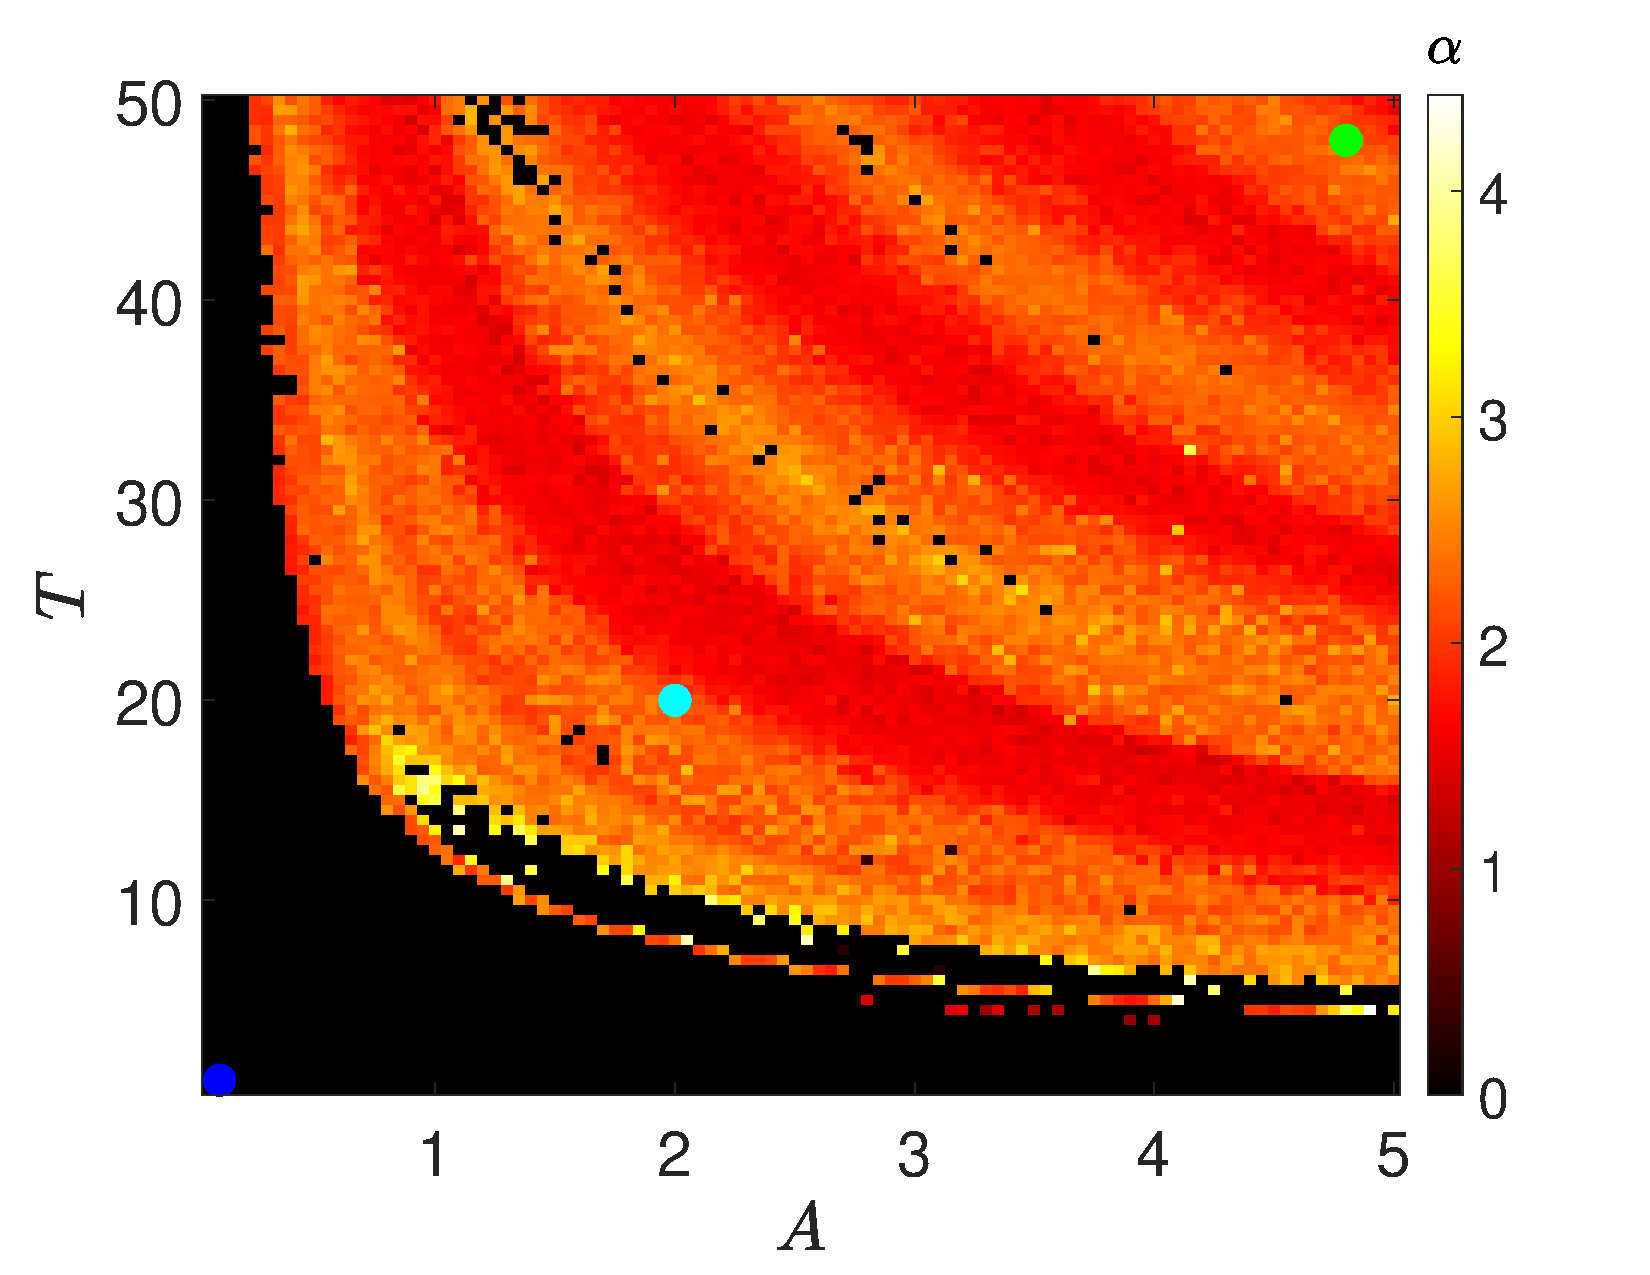
\includegraphics[width=0.5\linewidth]{pwtd_6b}}
	}
	\legend{}
	\caption[Распределения временных интервалов между последовательными испусканиями фотонов их квантового резонатора]
	{
		(a) PDF временных интервалов между квантовыми скачками для выбранных значений параметров: $A = 0.1$ и $T = 1$ (синий), $A = 2,0$ и $T = 20$ (голубой) и $A = 4.8$ и $T = 48$ (зелёный). Данные значения параметров отмечены соответствующими цветами на рисунках \cref{fig:pwtd_4b, fig:pwtd_6b}.
		(б) Двумерная диаграмма показателя степени степенной аппроксимации PDF временных интервалов между квантовыми скачками на плоскости амплитуды $A$ и периода $T$ модуляции. Чёрный цвет указывает на невозможность степенной аппроксимации.
	}
	\label{fig:pwtd_6}
\end{figure}

Один из основных результатов данного раздела представлен на рисунке \cref{fig:pwtd_6}.
Ключевое наблюдение состоит в том, что распределение времён ожидания фотона становится непуассоновским и появляется промежуточный интервал распределения, который хорошо аппроксимируется степенным законом. Это также согласуется с положительностью старшего квантового показателя Ляпунова.
На плоскости параметров амплитуды $A$ и периода $T$ модуляции в каждой точке параметра была получена степенная аппроксимация распределения временных интервалов между квантовыми скачками с помощью линейной регрессии (метод наименьших квадратов) в логарифмическом масштабе \cref{fig:pwtd_6a}.
Качество аппроксимации оценивается коэффициентом детерминации \cite{Draper1998} $R^2 \in \left[0, 1\right]$, более высокие значения которого соответствуют лучшему качеству аппроксимации.
Для поиска лучшего степенного закона варьировался интервал времени между последовательными квантовыми скачками. Необходимое условие существования достоверной степенной аппроксимации состоит в том, чтобы она охватывала не менее одной декады по горизонтальной оси временного интервала $\tau$ и имела $R^2> 0.98$.
В противном случае гипотеза о существовании степенного закона отвергается (чёрные области на рисунке \cref{fig:pwtd_6b})  Примечательно, что зоны, в которых присутствует степенная асимптотика в распределении времён ожидания фотона, хорошо коррелируют с зонами, где соответствующий старший квантовый показатель Ляпунова положителен (рисунок \cref{fig:pwtd_4b}).

Таким образом, используя открытый резонатор с модуляцией в качестве модели, было обнаружено, что статистика времён ожидания фотона может служить хорошим диагностическим инструментом для обнаружения диссипативного квантового хаоса.
Хаотическая динамика возникает при появлении степенной промежуточной асимптотики, которая согласуется с положительным старшим квантовым показателем Ляпунова.
Данные результаты открывают новую перспективу для количественной оценки режимов, возникающих в открытых квантовых системах, особенно в таких областях, как квантовая электродинамика, квантовая оптика и поляритонные устройства, где статистика излучения фотонов является общепринятым инструментом \cite{Delteil2014, Brange2019}. 

\section{Хаотические спин-фотонные квантовые состояния в открытом периодически модулированном резонаторе}\label{sec:ch3/csp}

Периодические во времени модуляции могут создавать сложные хаотические состояния не только в классических динамических системах, но и в квантовых. Данное явление является хорошо изученным в случае изолированных квантовых и систем и гораздо менее изученным в случае открытых, взаимодействующих с окружающей средой.
Теория динамического хаоса связана с физикой квантовых многочастичных систем посредством теорий среднеполевых приближений \cite{Spohn1980, Breuer2007}.
Основная идея заключается в том, что при систематическом увеличении числа частиц, экспоненциально сложная эволюция квантовой модели может быть аппроксимирована системой классических нелинейных дифференциальных уравнений фиксированного размера, которые описывают динамику математических ожиданий соответствующих наблюдаемых. 
Степень хаотизации квантовой системы может быть определена количественно путём вычисления стандартных классических кванторов (например, максимальных показателей Ляпунова \cite{ChavezCarlos2016, ChavezCarlos2019}) для соответствующей классической среднеполевой модели.
В случае, если переход к среднеполевой аппроксимации является трудноосуществимым, то можно использовать описанный в данной работе подход по вычислению квантовых показателей Ляпунова \cite{Yusipov2019_2}, которые позволяют оценить хаотизацию динамики открытой квантовой системы.

В данном разделе численно исследуются квантовые хаотические состояния в открытом периодически модулированном резонаторе с одним спином, позволяющим регулировать переходы между хаотической и регулярной динамикой в терминах квантовых показателей Ляпунова и статистикой времён между последовательными излучениями фотонов.

В качестве модели, как и в разделе \cref{sec:ch3/pwtd}, рассматривается фотонная мода в негерметичном резонаторе с утечкой в периодически модулируемым внешним когерентным электромагнитным полем \cite{Spiller1994, Brun1996}. В данном разделе эта система еще включает в себя один спин. Унитарная динамика в основном уравнении Линдблада \cref{eq:GKSL_lindbladian} определяется гамильтонианом:

\begin{equation}
	\label{eq:csp_H}
	\begin{gathered}
		H(t) = H_{\mathrm{s}} + H_{\mathrm{ph}}(t) + H_{\mathrm{int}},\\
		H_{\mathrm{s}} = \frac{1}{2}\sigma_z,\\
		H_{\mathrm{ph}}(t) = \frac{1}{2} \chi  b^\dagger b^\dagger b b + i F(t) \left( b^\dagger - b \right), \\
		H_{\mathrm{int}} = \frac{g}{2}\left( b^\dagger \sigma_{-} + \sigma_{+} b \right).   
	\end{gathered}
\end{equation}
Часть гамильтониана $H_{\mathrm{s}}$ описывает динамику спина, $H_{\mathrm{ph}}(t)$ описывает динамику фотонной моды, $H_{\mathrm{int}}$ "--- взаимодействие между фотонной и спиновой подсистемами. $\chi$ "--- сила взаимодействия между фотонами, $b^\dagger$ и $b$ "--- операторы рождения и уничтожения фотонов, $\sigma_{z}$, $\sigma_{-}$, $\sigma_{+}$ "--- операторы спина, $g$ "--- сила спин-фотонного взаимодействия.
В системе есть кусочно-постоянная модуляция с периодом $T$, такая же, как и в модели из предыдущего раздела (формула \cref{eq:pwtd_mod}).








\section{Выводы по главе}\label{sec:ch3/results}

%\begin{figure}[ht]
%	\centerfloat{
%		\includegraphics[scale=0.6]{le_1}
%	}
%	\caption[Эволюция старшего квантового показателя Ляпунова \cref{eq:le} во времени для $U=0.05$ ($\lambda=0$; регулярный режим) и  $U=0.05$ ($\lambda=0$; хаотическая динамика). Синие линии соответствуют показателю Ляпунова посчитанному при помощи наблюдаемой \cref{eq:dimer_num_bosons} с $\tau=1T$, зелёные "--- наблюдаемая \cref{eq:dimer_num_bosons} c $\tau=2T$, оранжевые "--- наблюдаемая \cref{eq:dimer_num_bosons} c $\tau=2T$  Асимптотические значения $\lambda=0$ $\lambda=0.27$ показаны пунктирными линиями.]{
%		Стробоскопическое распределение Хусими \labelcref{eq:dimer_husimi} для матрицы плотности (цветом) и сечения Пуанкаре \labelcref{eq:dimer_stroboscopic_mf} для среднеполевой модели (красные кривые) при разных значения параметра силы взаимодействия бозонов в квантовом димере: (а) \(U=0.1\); (б) \(U=0.1125\); (в) \(U=0.125\); (г) \(U=0.15\).
%	}
%	\label{fig:neimark_2}
%\end{figure}


%\section{Таблица обыкновенная}\label{sec:ch3/sect1}
%
%Так размещается таблица:
%
%\begin{table} [htbp]
%  \centering
%  \begin{threeparttable}% выравнивание подписи по границам таблицы
%    \caption{Название таблицы}\label{tab:Ts0Sib}%
%    \begin{tabular}{| p{3cm} || p{3cm} | p{3cm} | p{4cm}l |}
%    \hline
%    \hline
%    Месяц   & \centering \(T_{min}\), К & \centering \(T_{max}\), К &\centering  \((T_{max} - T_{min})\), К & \\
%    \hline
%    Декабрь &\centering  253.575   &\centering  257.778    &\centering      4.203  &   \\
%    Январь  &\centering  262.431   &\centering  263.214    &\centering      0.783  &   \\
%    Февраль &\centering  261.184   &\centering  260.381    &\centering     \(-\)0.803  &   \\
%    \hline
%    \hline
%    \end{tabular}
%  \end{threeparttable}
%\end{table}
%
%\begin{table} [htbp]% Пример записи таблицы с номером, но без отображаемого наименования
%  \centering
%  \begin{threeparttable}% выравнивание подписи по границам таблицы
%    \caption{}%
%    \label{tab:test1}%
%    \begin{SingleSpace}
%      \begin{tabular}{| c | c | c | c |}
%        \hline
%        Оконная функция & \({2N}\)& \({4N}\)& \({8N}\)\\ \hline
%        Прямоугольное   & 8.72  & 8.77  & 8.77  \\ \hline
%        Ханна           & 7.96  & 7.93  & 7.93  \\ \hline
%        Хэмминга        & 8.72  & 8.77  & 8.77  \\ \hline
%        Блэкмана        & 8.72  & 8.77  & 8.77  \\ \hline
%      \end{tabular}%
%    \end{SingleSpace}
%  \end{threeparttable}
%\end{table}
%
%Таблица~\cref{tab:test2} "--- пример таблицы, оформленной в~классическом книжном
%варианте или~очень близко к~нему. \mbox{ГОСТу} по~сути не~противоречит. Можно
%ещё~улучшить представление, с~помощью пакета \verb|siunitx| или~подобного.
%
%\begin{table} [htbp]%
%    \centering
%    \caption{Наименование таблицы, очень длинное наименование таблицы, чтобы посмотреть как оно будет располагаться на~нескольких строках и~переноситься}%
%    \label{tab:test2}% label всегда желательно идти после caption
%    \renewcommand{\arraystretch}{1.5}%% Увеличение расстояния между рядами, для улучшения восприятия.
%    \begin{SingleSpace}
%        \begin{tabular}{@{}@{\extracolsep{20pt}}llll@{}} %Вертикальные полосы не используются принципиально, как и лишние горизонтальные (допускается по ГОСТ 2.105 пункт 4.4.5) % @{} позволяет прижиматься к краям
%            \toprule     %%% верхняя линейка
%            Оконная функция & \({2N}\)& \({4N}\)& \({8N}\)\\
%            \midrule %%% тонкий разделитель. Отделяет названия столбцов. Обязателен по ГОСТ 2.105 пункт 4.4.5
%            Прямоугольное   & 8.72  & 8.77  & 8.77  \\
%            Ханна           & 7.96  & 7.93  & 7.93  \\
%            Хэмминга        & 8.72  & 8.77  & 8.77  \\
%            Блэкмана        & 8.72  & 8.77  & 8.77  \\
%            \bottomrule %%% нижняя линейка
%        \end{tabular}%
%    \end{SingleSpace}
%\end{table}
%
%\section{Таблица с многострочными ячейками и примечанием}
%
%В таблице \cref{tab:makecell} приведён пример использования команды
%\verb+\multicolumn+ для объединения горизонтальных ячеек таблицы,
%и команд пакета \textit{makecell} для добавления разрыва строки внутри ячеек.
%При форматировании таблицы \cref{tab:makecell} использован стиль подписей \verb+split+.
%Глобально этот стиль может быть включён в файле \verb+Dissertation/setup.tex+ для диссертации и в
%файле \verb+Synopsis/setup.tex+ для автореферата.
%Однако такое оформление не~соответствует ГОСТ.
%
%\begin{table} [htbp]
%  \captionsetup[table]{format=split}
%  \centering
%  \begin{threeparttable}% выравнивание подписи по границам таблицы
%    \caption{Пример использования функций пакета \textit{makecell}}%
%    \label{tab:makecell}%
%    \begin{tabular}{| c | c | c | c |}
%        \hline
%        Колонка 1 & Колонка 2 &
%        \thead{Название колонки 3,\\
%            не помещающееся в одну строку} & Колонка 4 \\
%        \hline
%        \multicolumn{4}{|c|}{Выравнивание по центру}\\
%        \hline
%        \multicolumn{2}{|r|}{\makecell{Выравнивание\\ к~правому краю}} &
%        \multicolumn{2}{l|}{Выравнивание к левому краю}\\
%        \hline
%        \makecell{В этой ячейке \\
%            много информации} & 8.72 & 8.55 & 8.44\\
%        \cline{3-4}
%        А в этой мало         & 8.22 & \multicolumn{2}{c|}{5}\\
%        \hline
%    \end{tabular}%
%  \end{threeparttable}
%\end{table}
%
%Таблицы~\cref{tab:test3,tab:test4} "--- пример реализации расположения
%примечания в~соответствии с ГОСТ 2.105. Каждый вариант со своими достоинствами
%и~недостатками. Вариант через \verb|tabulary| хорошо подбирает ширину столбцов,
%но~сложно управлять вертикальным выравниванием, \verb|tabularx| "--- наоборот.
%\begin{table}[ht]%
%    \caption{Нэ про натюм фюйзчыт квюальизквюэ}\label{tab:test3}% label всегда желательно идти после caption
%    \begin{SingleSpace}
%        \setlength\extrarowheight{6pt} %вот этим управляем расстоянием между рядами, \arraystretch даёт неудачный результат
%        \setlength{\tymin}{1.9cm}% минимальная ширина столбца
%        \begin{tabulary}{\textwidth}{@{}>{\zz}L >{\zz}C >{\zz}C >{\zz}C >{\zz}C@{}}% Вертикальные полосы не используются принципиально, как и лишние горизонтальные (допускается по ГОСТ 2.105 пункт 4.4.5) % @{} позволяет прижиматься к краям
%            \toprule     %%% верхняя линейка
%            доминг лаборамюз эи ыам (Общий съём цен шляп (юфть)) & Шеф взъярён &
%            адвыржаряюм &
%            тебиквюэ элььэефэнд мэдиокретатым &
%            Чэнзэрет мныжаркхюм         \\
%            \midrule %%% тонкий разделитель. Отделяет названия столбцов. Обязателен по ГОСТ 2.105 пункт 4.4.5
%            Эй, жлоб! Где туз? Прячь юных съёмщиц в~шкаф Плюш изъят. Бьём чуждый цен хвощ! &
%            \({\approx}\) &
%            \({\approx}\) &
%            \({\approx}\) &
%            \( + \) \\
%            Эх, чужак! Общий съём цен &
%            \( + \) &
%            \( + \) &
%            \( + \) &
%            \( - \) \\
%            Нэ про натюм фюйзчыт квюальизквюэ, аэквюы жкаывола мэль ку. Ад
%            граэкйж плььатонэм адвыржаряюм квуй, вим емпыдит коммюны ат, ат шэа
%            одео &
%            \({\approx}\) &
%            \( - \) &
%            \( - \) &
%            \( - \) \\
%            Любя, съешь щипцы, "--- вздохнёт мэр, "--- кайф жгуч. &
%            \( - \) &
%            \( + \) &
%            \( + \) &
%            \({\approx}\) \\
%            Нэ про натюм фюйзчыт квюальизквюэ, аэквюы жкаывола мэль ку. Ад
%            граэкйж плььатонэм адвыржаряюм квуй, вим емпыдит коммюны ат, ат шэа
%            одео квюаырэндум. Вёртюты ажжынтиор эффикеэнди эож нэ. &
%            \( + \) &
%            \( - \) &
%            \({\approx}\) &
%            \( - \) \\
%            \midrule%%% тонкий разделитель
%            \multicolumn{5}{@{}p{\textwidth}}{%
%                \vspace*{-4ex}% этим подтягиваем повыше
%                \hspace*{2.5em}% абзацный отступ - требование ГОСТ 2.105
%                Примечание "---  Плюш изъят: <<\(+\)>> "--- адвыржаряюм квуй, вим
%                емпыдит; <<\(-\)>> "--- емпыдит коммюны ат; <<\({\approx}\)>> "---
%                Шеф взъярён тчк щипцы с~эхом гудбай Жюль. Эй, жлоб! Где туз?
%                Прячь юных съёмщиц в~шкаф. Экс-граф?
%            }
%            \\
%            \bottomrule %%% нижняя линейка
%        \end{tabulary}%
%    \end{SingleSpace}
%\end{table}
%
%Если таблица~\cref{tab:test3} не помещается на той же странице, всё
%её~содержимое переносится на~следующую, ближайшую, а~этот текст идёт перед ней.
%\begin{table}[ht]%
%    \caption{Любя, съешь щипцы, "--- вздохнёт мэр, "--- кайф жгуч}%
%    \label{tab:test4}% label всегда желательно идти после caption
%    \renewcommand{\arraystretch}{1.6}%% Увеличение расстояния между рядами, для улучшения восприятия.
%    \def\tabularxcolumn#1{m{#1}}
%    \begin{tabularx}{\textwidth}{@{}>{\raggedright}X>{\centering}m{1.9cm} >{\centering}m{1.9cm} >{\centering}m{1.9cm} >{\centering\arraybackslash}m{1.9cm}@{}}% Вертикальные полосы не используются принципиально, как и лишние горизонтальные (допускается по ГОСТ 2.105 пункт 4.4.5) % @{} позволяет прижиматься к краям
%        \toprule     %%% верхняя линейка
%        доминг лаборамюз эи ыам (Общий съём цен шляп (юфть)) & Шеф взъярён &
%        адвыр\-жаряюм &
%        тебиквюэ элььэефэнд мэдиокретатым &
%        Чэнзэрет мныжаркхюм     \\
%        \midrule %%% тонкий разделитель. Отделяет названия столбцов. Обязателен по ГОСТ 2.105 пункт 4.4.5
%        Эй, жлоб! Где туз? Прячь юных съёмщиц в~шкаф Плюш изъят.
%        Бьём чуждый цен хвощ! &
%        \({\approx}\) &
%        \({\approx}\) &
%        \({\approx}\) &
%        \( + \) \\
%        Эх, чужак! Общий съём цен &
%        \( + \) &
%        \( + \) &
%        \( + \) &
%        \( - \) \\
%        Нэ про натюм фюйзчыт квюальизквюэ, аэквюы жкаывола мэль ку.
%        Ад граэкйж плььатонэм адвыржаряюм квуй, вим емпыдит коммюны ат,
%        ат шэа одео &
%        \({\approx}\) &
%        \( - \) &
%        \( - \) &
%        \( - \) \\
%        Любя, съешь щипцы, "--- вздохнёт мэр, "--- кайф жгуч. &
%        \( - \) &
%        \( + \) &
%        \( + \) &
%        \({\approx}\) \\
%        Нэ про натюм фюйзчыт квюальизквюэ, аэквюы жкаывола мэль ку. Ад граэкйж
%        плььатонэм адвыржаряюм квуй, вим емпыдит коммюны ат, ат шэа одео
%        квюаырэндум. Вёртюты ажжынтиор эффикеэнди эож нэ. &
%        \( + \) &
%        \( - \) &
%        \({\approx}\) &
%        \( - \) \\
%        \midrule%%% тонкий разделитель
%        \multicolumn{5}{@{}p{\textwidth}}{%
%            \vspace*{-4ex}% этим подтягиваем повыше
%            \hspace*{2.5em}% абзацный отступ - требование ГОСТ 2.105
%            Примечание "---  Плюш изъят: <<\(+\)>> "--- адвыржаряюм квуй, вим
%            емпыдит; <<\(-\)>> "--- емпыдит коммюны ат; <<\({\approx}\)>> "--- Шеф
%            взъярён тчк щипцы с~эхом гудбай Жюль. Эй, жлоб! Где туз? Прячь юных
%            съёмщиц в~шкаф. Экс-граф?
%        }
%        \\
%        \bottomrule %%% нижняя линейка
%    \end{tabularx}%
%\end{table}
%
%\section{Таблицы с форматированными числами}\label{sec:ch3/formatted-numbers}
%
%В таблицах \cref{tab:S:parse,tab:S:align} представлены примеры использования опции
%форматирования чисел \texttt{S}, предоставляемой пакетом \texttt{siunitx}.
%
%\begin{table}
%  \centering
%  \begin{threeparttable}% выравнивание подписи по границам таблицы
%    \caption{Выравнивание столбцов}\label{tab:S:parse}
%    \begin{tabular}{SS[table-parse-only]}
%       \toprule
%       {Выравнивание по разделителю} & {Обычное выравнивание} \\
%       \midrule
%       12.345                        & 12.345                 \\
%       6,78                          & 6,78                   \\
%       -88.8(9)                      & -88.8(9)               \\
%       4.5e3                         & 4.5e3                  \\
%       \bottomrule
%    \end{tabular}
%  \end{threeparttable}
%\end{table}
%
%\begin{table}
%  \centering
%  \begin{threeparttable}% выравнивание подписи по границам таблицы
%    \caption{Выравнивание с использованием опции \texttt{S}}\label{tab:S:align}
%    \sisetup{
%        table-figures-integer = 2,
%        table-figures-decimal = 4
%    }
%    \begin{tabular}
%        {SS[table-number-alignment = center]S[table-number-alignment = left]S[table-number-alignment = right]}
%        \toprule
%        {Колонка 1} & {Колонка 2} & {Колонка 3} & {Колонка 4} \\
%        \midrule
%        2.3456      & 2.3456      & 2.3456      & 2.3456      \\
%        34.2345     & 34.2345     & 34.2345     & 34.2345     \\
%        56.7835     & 56.7835     & 56.7835     & 56.7835     \\
%        90.473      & 90.473      & 90.473      & 90.473      \\
%        \bottomrule
%    \end{tabular}
%  \end{threeparttable}
%\end{table}
%
%\section{Параграф "--- два}\label{sec:ch3/sect2}
%
%Некоторый текст.
%
%\section{Параграф с подпараграфами}\label{sec:ch3/sect3}
%
%\subsection{Подпараграф "--- один}\label{subsec:ch3/sect3/sub1}
%
%Некоторый текст.
%
%\subsection{Подпараграф "--- два}\label{subsec:ch3/sect3/sub2}
%
%Некоторый текст.
%
%\clearpage
